\chapter{基于多方向表征建模的幻觉检测方法}\label{chp:chapter3}

% 第一项研究内容针对现有幻觉检测方法部分方法依赖标注训练数据集导致泛化差的问题，本文拟从大语言模型生成过程中的隐藏状态与激活表示出发，研究一种\emph{基于多方向表征建模的幻觉检测方法}。其具体贡献如下：

% \begin{itemize}
%     \item 提出一种基于多方向表征建模的幻觉检测方法ATScore（Activation Tensor Score）。利用多方向链式表征建模深入探索大语言模型内部表征的演化结构，从而高效地利用模型内部表征的动态变化特征，构建更稳定、有效且免于训练的幻觉检测信号，同时保证检测的低开销和良好的跨模型、跨领域泛化能力。
%     \item ATScore提出在三维激活张量的统一视角下看待跨层和跨token方向的表征信息，从两个维度挖掘模型内部表征中蕴含的幻觉线索，最终实现对内部各位置表征信息的充分利用。
%     \item 在多个开源大模型和公开幻觉检测数据集上进行全面评估，并针对多种算法变体进行多种消融实验，验证所提出方法在不同模型、不同任务和不同领域上的有效性与泛化能力。与现有主流方法进行对比分析，展示其在提升幻觉检测准确性、稳定性以及跨场景适用性方面的优势。
% \end{itemize}

现有幻觉检测方法虽然已取得一定进展，但其中相当一部分方法依赖标注训练数据集来学习判别信号，因而在跨数据集、跨场景甚至跨模型设置下往往面临泛化能力受限的问题。相比之下，大语言模型生成过程中的内部表征蕴含了更丰富的中间语义与推理信息，有望为构造无需额外训练、具备更强泛化能力的幻觉检测信号提供新的切入点。然而，如何有效挖掘并利用这些内部表征，仍是当前研究中的一个关键问题。

本章针对现有幻觉检测方法依赖标注训练数据集、导致泛化能力受限的问题，提出ATScore（Activation Tensor Score）算法。该方法在三维激活张量的统一视角下刻画大语言模型内部表征，并沿跨层与跨词元两个方向进行链式建模，从而从内部表征演化过程中挖掘与幻觉相关的异常线索，构造一种无需额外训练的白盒幻觉检测信号。

\section{问题设定}

本文采用当前较为主流且实现简便的大模型幻觉检测问题定义。给定一个大模型$M$、一段用户输入文本的词元（token）序列$X=\{x_1, x_2, \ldots, x_n\}$及其对应的标准答案$Z=\{z_1, z_2, \ldots, z_k\}$，以及模型生成的输出文本token序列$Y=\{y_1, y_2, \ldots, y_m\}$，其中$n$、$k$和$m$分别表示对应序列中的token数量。幻觉检测任务的目标是判断模型生成的输出文本$Y$中是否包含幻觉内容，即判断其是否与标准答案$Z$在语义上保持一致。

从形式上看，幻觉检测可以建模为一个简单的二分类问题，其目标是学习一个判别函数$f(M, X, Y) \rightarrow \{0, 1\}$，其中，$f$表示幻觉检测模型。当输出为1时，表示模型输出中存在幻觉内容；当输出为0时，表示模型输出中不存在幻觉内容。换言之，该任务关注的是模型输出的事实正确性或语义一致性，而非仅仅关注其语言表达是否流畅自然。

在白盒设定下，除了模型生成的输出文本$Y$之外，大模型在生成过程中产生的一系列内部隐藏状态同样是可获取的。此时，幻觉检测问题可以建模为：
\begin{equation}
f(M,X,Y,H)\rightarrow \{0,1\},
\end{equation}
其中$H$表示模型在生成过程中得到的内部表征集合。这些内部表征包含了模型在不同层、不同token位置上的中间语义信息，因此也可以作为额外输入提供给幻觉检测模型，以辅助判断模型输出的幻觉程度。相比仅依赖最终输出文本的黑盒设定，白盒设定能够更加充分地利用模型内部信息，为幻觉检测提供更丰富的判别依据。

进一步地，关于“模型输出是否与标准答案一致”的判定方式，需要结合具体数据集的任务形式来确定。在封闭式问题设定中，例如选择题、判断题等任务，模型输出通常具有较为明确的标准形式。此时，可以先利用正则表达式等工具对模型输出进行解析，再将解析结果与标准答案进行直接比较，从而判断模型是否回答正确。由于此类任务答案空间相对有限，因此判定标准通常较为直接。

而在开放式问题设定中，例如问答任务、开放生成任务等，模型输出往往具有较强的表达多样性。即使模型输出与标准答案在语义上相符，其表面形式也可能存在较大差异。因此，在这类场景下，通常需要采用更复杂的评判标准，以避免仅依据字面匹配造成误判。常见的评判方式包括基于文本相似度的自动评判方法，如BLEU（Bilingual Evaluation Understudy）\cite{papineni2002bleu}、ROUGE（Recall-Oriented Understudy for Gisting Evaluation）\cite{lin2004rouge}、BERTScore\cite{zhang2020bertscore}等；此外，也可以采用基于人工标注或更强大模型评判的方式。例如，可将标准答案与模型输出按照预设模板进行拼接，并输入到具有较高知识能力的大模型中，由其给出“相符”或“不相符”的判断结果。

综上所述，幻觉检测任务的核心在于建立从模型、输入与输出到幻觉标签之间的映射关系，而具体的一致性判定方式则依赖于任务形式与数据集特征。在本章实验中，本文将根据不同数据集的具体特点，选取与其任务形式相适应的评判标准，以保证幻觉检测任务定义的合理性与实验结论的有效性。

\section{ATScore算法}

本方法属于无需训练的白盒幻觉检测方法，核心思想是从大语言模型内部表征中构建三维激活张量，并在该统一视角下挖掘跨层和跨token方向的幻觉线索，最终构建一个稳定、有效且免于训练的幻觉检测信号。本方法的框架结构图如图~\ref{fig:atscore_overview}所示。后续章节将按步骤详细介绍ATScore算法的设计与实现。

\begin{figure}[htbp]
    \centering
    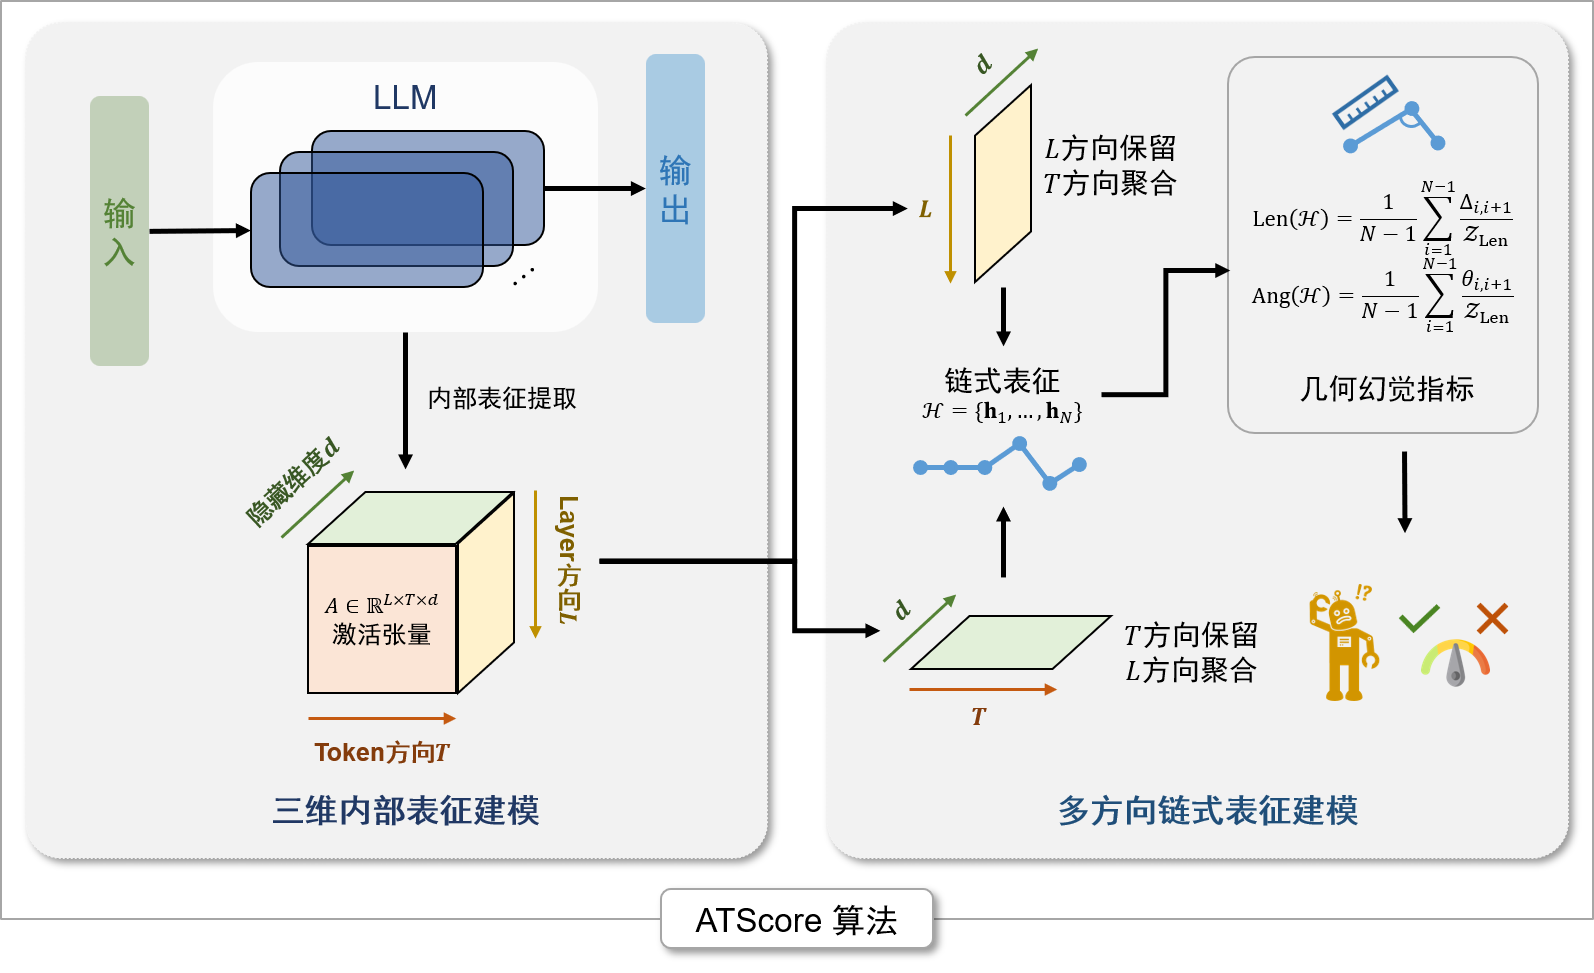
\includegraphics[width=\textwidth]{figures/content/第三章方法总览.png}
    \caption{ATScore算法框架图}\label{fig:atscore_overview}
\end{figure}

\subsection{三维内部表征建模}

在大语言模型的生成过程中，隐藏状态不仅在层间逐步演化，同时也随着生成序列在时间维度上不断展开。因此，如何从多维度刻画内部表征的动态变化，对于识别潜在的幻觉信号具有重要意义。模型在生成过程中产生的不稳定或异常表征，往往可以通过隐藏状态的结构性变化体现出来。为系统刻画这一过程，本文采用与已有工作\cite{bar2025beyond}一致的内部表征提取方式，并在此基础上进行统一建模。具体而言，本文定义“激活张量（Activation Tensor）”为$\mathbf{A} \in \mathbb{R}^{L \times T \times d}$，其中$L$表示Transformer的层数，$T$表示生成输出文本的token数量，$d$表示每层隐藏状态的维度。

具体地，对于生成输出序列中的每一个token $y_t$（$t = 1, 2, \ldots, T$），提取模型在生成该token时各层Transformer模块的隐藏状态，即
\begin{equation}
\mathbf{A}_{:,t,:} = \{ \mathbf{a}_{1,t}, \mathbf{a}_{2,t}, \ldots, \mathbf{a}_{L,t} \}.
\end{equation}
其中$\mathbf{a}_{\ell,t} \in \mathbb{R}^d$表示第$\ell$层在生成第$t$个token时的隐藏状态向量。通过对所有token重复该过程，可以构建完整的三维激活张量$\mathbf{A}$，从而同时保留跨层（layer-wise）与跨token（token-wise）的表征信息。

与仅关注单层或单token位置的局部表示不同，该三维张量提供了一种更加结构化的视角，使得从不同维度刻画模型内部表征的变化模式成为可能。例如，沿layer维度可以刻画信息在网络深度方向上的传播过程，而沿token维度则反映生成序列随时间展开的语义演化轨迹。这种多维结构为后续挖掘幻觉相关信号提供了更丰富的信息基础。

在此基础上，本文进一步引入“链式表示”的概念，将高维激活张量在特定方向上展开为一系列有序的向量序列，从而将复杂的三维表征结构转化为可分析的表示演化轨迹。具体的链式构建方式将在下一小节中进行详细介绍。

\subsection{多方向链式表征建模}\label{subsec:multi_direction_chain_representation}

现有研究已经表明，将隐藏状态在某一方向上组织为有序向量序列，有助于刻画大语言模型在推理过程中的潜在表示变化轨迹\cite{wang2025latent}。受此启发，本文进一步提出多方向链式表征建模方法，即在激活张量的两个正交方向上分别构造链式表示，从不同视角刻画内部表征的演化模式。与仅关注单一层、单一token位置的静态探测方式不同，该建模方式能够将三维内部表征转化为可分析的表示轨迹，从而更充分地利用大模型内部状态中与幻觉相关的动态信息。

\subsubsection{链式表征的基本定义}

设$\mathbf{a}_{\ell,t} \in \mathbb{R}^{d}$表示激活张量中第$\ell$层、第$t$个token对应的隐藏状态向量，其中$\ell = 1,2,\dots,L$，$t = 1,2,\dots,T$。链式表征的目标是将原始的三维张量映射为一条由若干embedding组成的有序链；为此，在保留某一主方向顺序结构的同时，需对另一辅助方向进行压缩聚合。从而形式上，若链中共有$N$个状态点，则可表示为
\begin{equation}
  \label{eq:chain_representation}
  \mathcal{H} = \{\mathbf{h}_1,\mathbf{h}_2,\dots,\mathbf{h}_N\}, \qquad \mathbf{h}_i \in \mathbb{R}^{d}.
\end{equation}
这里，$\mathcal{H}$中的每一个状态向量$\mathbf{h}_i$可视为三维激活张量$A$在某一主方向位置上、融合另一辅助方向信息后得到的表征摘要。由于这些状态向量具有天然的顺序关系，因此可以进一步视为潜在表示空间中的一条离散轨迹。类似于人类大脑思考问题时的逻辑链，这些状态向量同样可以在某种程度上视为是大模型的“思维链”。本文的基本假设是：当模型生成事实一致、语义可靠的内容时，其内部表示轨迹通常更平滑、更稳定，并呈现出不同于幻觉生成样本的几何特征；相反，当模型生成幻觉内容时，内部状态往往会出现异常的跳变、偏折或不一致性，这些差异可以通过链式表征的几何统计量加以刻画。

基于“主方向--辅助方向”的建模思想，本文考虑如下两类互补的链式构造方式。

\subsubsection{基于layer主方向的链式表征}

第一类链式表征以layer为主方向，即保持网络深度方向上的顺序结构，同时对token方向的信息进行聚合。该方式与已有工作\cite{wang2025latent}中从层间表示演化角度刻画模型内部状态的思路一致，其关注的是：对于同一段生成文本，模型的整体句子级表示如何随着网络层数逐步变化。

具体而言，对于第$\ell$层的所有token隐藏状态$\{\mathbf{a}_{\ell,1},\mathbf{a}_{\ell,2},\dots,\mathbf{a}_{\ell,T}\}$，本文在token方向采用聚合算子$\phi_t(\cdot)$，得到该层对应的链状态
\begin{equation}
  \mathbf{h}^{(\mathrm{layer})}_{\ell} = \phi_t\big(\mathbf{a}_{\ell,1},\mathbf{a}_{\ell,2},\dots,\mathbf{a}_{\ell,T}\big), \quad \ell = 1,2,\dots,L.
\end{equation}
于是可得到一条长度为$L$的layer链
\begin{equation}
  \mathcal{H}^{(\mathrm{layer})}
  =
  \left\{
  \mathbf{h}^{(\mathrm{layer})}_{1},
  \mathbf{h}^{(\mathrm{layer})}_{2},
  \dots,
  \mathbf{h}^{(\mathrm{layer})}_{L}
  \right\}.
\end{equation}
其中，token方向的聚合算子$\phi_t(\cdot)$可以有多种实现方式。本文重点考虑如下两种简单而有效的无参数聚合方式：$\phi_t^{\mathrm{avg}}=\frac{1}{T}\sum_{t=1}^{T}\mathbf{a}_{\ell,t}$，即对该层所有token隐藏状态取平均，以获得句子级全局表示；以及$\phi_t^{\mathrm{last}}=\mathbf{a}_{\ell,T}$，即取最后一个输出token对应的隐藏状态，以强调生成末端的决策信息。前者更关注整体语义摘要，后者则更接近许多语言模型中常用的末位置表征方式。因大模型的逐token输出特性，末token通常能够携带更多的上下文信息，适于用作句子级表征。通过比较不同聚合方式，能够考察辅助方向压缩策略对链式几何特征的影响。

\subsubsection{基于token主方向的链式表征}

与上述方法不同，本文更关注另一种对偶但尚未被充分研究的建模视角，即以token为主方向构建链式表征，同时对layer方向进行聚合。该方式保留了生成序列随时间展开的顺序结构，关注的是：在整个生成过程中，每个位置上的表示在融合多层信息后如何形成一条沿输出序列推进的潜在语义轨迹。

具体而言，对于第$t$个token在所有层上的隐藏状态$\{\mathbf{a}_{1,t},\mathbf{a}_{2,t},\dots,\mathbf{a}_{L,t}\}$，本文在layer方向采用聚合算子$\phi_{\ell}(\cdot)$，得到该token对应的链状态
\begin{equation}
  \mathbf{h}^{(\mathrm{token})}_{t}
  =
  \phi_{\ell}\big(\mathbf{a}_{1,t},\mathbf{a}_{2,t},\dots,\mathbf{a}_{L,t}\big), \qquad t = 1,2,\dots,T,
\end{equation}
从而构造出一条长度为$T$的token链
\begin{equation}
  \mathcal{H}^{(\mathrm{token})}
  =
  \left\{
  \mathbf{h}^{(\mathrm{token})}_{1},
  \mathbf{h}^{(\mathrm{token})}_{2},
  \dots,
  \mathbf{h}^{(\mathrm{token})}_{T}
  \right\}.
\end{equation}
类似于基于layer主方向的链式表征，layer方向的聚合算子$\phi_{\ell}(\cdot)$也可采用无参数聚合方式实现，例如$\phi_{\ell}^{\mathrm{avg}}=\frac{1}{L}\sum_{\ell=1}^{L}\mathbf{a}_{\ell,t}$以及$\phi_{\ell}^{\mathrm{last}}=\mathbf{a}_{L,t}$。类似于人类大脑中语言思维发展的方向，与沿layer方向构链相比，沿token方向构链能够更直接地刻画生成过程中的逐步语义推进与局部状态变化，因此对于识别“模型在何处开始偏离事实约束”这一问题具有更强的刻画能力。这也是本文相较于已有链式表征方法的重要区别之一。

\subsubsection{辅助方向聚合的可能变体}

除了上述avg与last两类基础聚合方式外，辅助方向的压缩还可以扩展为更多变体。例如，可以仅对中间若干层进行平均，以突出模型内部较稳定的语义表征；也可以对前后若干token进行局部窗口聚合，以降低极端位置噪声对链式表征的影响；还可以引入加权平均形式，使不同层或不同token在聚合时具有不同贡献。若记辅助方向上的若干隐藏状态为$\{\mathbf{v}_1,\mathbf{v}_2,\dots,\mathbf{v}_m\}$，则更一般的聚合形式可写为
\begin{equation}
\phi(\mathbf{v}_1,\dots,\mathbf{v}_m)
=
\sum_{i=1}^{m} w_i \mathbf{v}_i, \quad \sum_{i=1}^{m} w_i = 1.
\end{equation}
其中$w_i$为预先设定或数据驱动得到的权重。本文主要采用无参数的last与avg两类聚合方式，一方面是因为其形式简单、计算代价低；另一方面也有助于避免额外训练参数带来的模型依赖性，从而更好地体现无需训练（training-free）方法在跨模型、跨领域设定下的泛化优势。本文以下实验部分若无特殊说明，默认采用last方式进行辅助方向聚合。本文将在~\ref{subsec:ablation}中探讨辅助方向聚合方式的选择。

\subsubsection{链式表征的几何指标构造}

链式表征$\mathcal{H}$可视为嵌入空间$\mathbb{R}^d$中的一条离散轨迹（discrete trajectory），其沿序列维度刻画了隐藏状态的演化过程。从这一视角出发，轨迹的几何性质（如路径长度与方向变化）能够反映表示的稳定性与一致性，从而为刻画生成过程中的潜在异常提供依据。为刻画链式表征的几何特性，本文关注两类统计量：路径长度用于衡量表示变化的幅度，转折角度用于刻画表示变化的方向稳定性。直观而言，语义一致的生成过程通常对应于平滑且稳定的表示轨迹，而幻觉生成过程则更可能表现为幅度波动或方向突变，因此上述几何指标能够有效区分两类生成模式。设链式表征为式~\ref{eq:chain_representation}所示，则第$i$个相邻状态对之间的位移长度可表示为
\begin{equation}
  \Delta_{i,i+1} = \|\mathbf{h}_{i+1}-\mathbf{h}_i\|_2, \quad i=1,2,\dots,N-1.
\end{equation}

首先，本文考虑链节点间的平均长度（chain length），用于衡量整条表示轨迹在潜在空间中的累计变化幅度：
\begin{equation}
  \label{eq:chain_length}
  \mathrm{Len}(\mathcal{H})
  =
  \frac{1}{N-1}\sum_{i=1}^{N-1}\frac{\Delta_{i,i+1}}{\mathcal{Z}_\mathrm{Len}}
  =
  \frac{1}{N-1}\sum_{i=1}^{N-1}\frac{\|\mathbf{h}_{i+1}-\mathbf{h}_i\|_2}{\mathcal{Z}_\mathrm{Len}}.
\end{equation}
其中$\mathcal{Z}_\mathrm{Len}$为归一化因子，定义为$\mathcal{Z}_\mathrm{Len}=\Delta_{1,N}=\|\mathbf{h}_{N}-\mathbf{h}_1\|_2$，即链的端到端距离。该指标越大，表示链在相邻状态之间的累计变化越剧烈，模型内部表征演化越不平稳。

进一步地，为刻画链式表征在方向上的折转程度，本文定义相邻表征向量之间的夹角。对于第$i$个内部节点，其对应的局部转角由余弦相似度的反三角函数得到，可写为
\begin{equation}
\theta_{i,i+1}
=
\arccos
\left(
\frac{
\mathbf{h}_{i+1}^{\top}\mathbf{h}_{i}
}{
\|\mathbf{h}_{i+1}\|_2\,\|\mathbf{h}_{i}\|_2
}
\right),
\quad i=1,2,\dots,N-1.
\end{equation}

在此基础上，可定义链的平均转折角度（turning angle）为
\begin{equation}
\mathrm{Ang}(\mathcal{H})
=
\frac{1}{N-1}
\sum_{i=1}^{N-1}\frac{\theta_{i,i+1}}{\mathcal{Z}_\mathrm{Ang}}.
\label{eq:chain_angle}
\end{equation}
其中$\mathcal{Z}_\mathrm{Ang}=\theta_{1,N}$为归一化因子，即链两端间的转折角，用于将角度变化标准化。该类指标反映了表示轨迹在局部方向上的频繁偏折程度。通常而言，若模型生成过程更加一致、连贯，其内部轨迹往往更平滑，对应较小的局部角度变化；而在生成幻觉内容时，模型可能在内部空间中出现更频繁的方向突变，从而表现出更大的弯曲度。

以上ATScore算法步骤总结于算法~\ref{alg:atscore}中，以便清晰地展示ATScore算法的整体流程。其中，当主方向为layer时，辅助方向聚合算子$\phi_t(\cdot)$可取token方向平均池化或末token池化；当主方向为token时，辅助方向聚合算子$\phi_{\ell}(\cdot)$可取layer方向平均池化或末层池化。

\begin{algorithm}[htb]
\caption{ATScore算法}
\label{alg:atscore}
\begin{algorithmic}[1]
\Require 激活张量$A\in\mathbb{R}^{L\times T\times d}$，其中$\mathbf{a}_{\ell,t}\in\mathbb{R}^d$；主方向$m\in\{\mathrm{layer},\mathrm{token}\}$；辅助方向聚合方式$\phi\in\{\mathrm{avg},\mathrm{last}\}$；几何指标类型$g\in\{\mathrm{Len},\mathrm{Ang}\}$
\Ensure 幻觉分数$s$

\If{$m=\mathrm{layer}$}
    \State $\mathbf{h}_{\ell}\gets \phi_t(\mathbf{a}_{\ell,1},\mathbf{a}_{\ell,2},\dots,\mathbf{a}_{\ell,T}),\ \ell=1,2,\dots,L$
    \State $\mathcal{H}\gets\{\mathbf{h}_1,\mathbf{h}_2,\dots,\mathbf{h}_L\},\quad N\gets L$
\Else
    \State $\mathbf{h}_{t}\gets \phi_{\ell}(\mathbf{a}_{1,t},\mathbf{a}_{2,t},\dots,\mathbf{a}_{L,t}),\ t=1,2,\dots,T$
    \State $\mathcal{H}\gets\{\mathbf{h}_1,\mathbf{h}_2,\dots,\mathbf{h}_T\},\quad N\gets T$
\EndIf

\For{$i=1,2,\dots,N-1$}
    \State $\Delta_{i,i+1}\gets \|\mathbf{h}_{i+1}-\mathbf{h}_i\|_2$
    \State $\theta_{i,i+1}\gets \arccos\!\left(\dfrac{\mathbf{h}_{i+1}^{\top}\mathbf{h}_i}{\|\mathbf{h}_{i+1}\|_2\,\|\mathbf{h}_i\|_2}\right)$
\EndFor

\State $\mathcal{Z}_{\mathrm{Len}}\gets \|\mathbf{h}_N-\mathbf{h}_1\|_2$
\State $\mathcal{Z}_{\mathrm{Ang}}\gets \arccos\!\left(\dfrac{\mathbf{h}_N^{\top}\mathbf{h}_1}{\|\mathbf{h}_N\|_2\,\|\mathbf{h}_1\|_2}\right)$

\If{$g=\mathrm{Len}$}
    \State $s\gets \dfrac{1}{N-1}\sum_{i=1}^{N-1}\dfrac{\Delta_{i,i+1}}{\mathcal{Z}_{\mathrm{Len}}}$
\Else
    \State $s\gets \dfrac{1}{N-1}\sum_{i=1}^{N-1}\dfrac{\theta_{i,i+1}}{\mathcal{Z}_{\mathrm{Ang}}}$
\EndIf

\State \Return $s$
\end{algorithmic}
\end{algorithm}

综上，本文通过在layer与token两个方向上构造互补的链式表征，并进一步提取链长、弯曲度、端到端位移及曲折程度等几何统计量。上述指标共同从幅值变化、方向变化和整体路径形态等多个方面刻画链式表征的几何属性，实现了从三维激活张量到低复杂度、可解释幻觉信号的映射。该建模方式不仅继承了链式表征对内部状态动态变化的刻画能力，还进一步扩展到token主方向建模视角，从而能够更系统地利用大语言模型内部表征中的多方向结构信息，为后续的幻觉检测打下基础。值得注意的是，本方法无需额外训练，直接从大模型内部参数中提取幻觉信号，其有效性基于如下观察：大语言模型在生成过程中，其隐藏状态已隐式编码了语义一致性与知识可靠性信息。通过对表示演化轨迹进行几何分析，可以直接从这些内部信号中提取与幻觉相关的判别特征，从而避免对额外监督数据的依赖，提升了可用性与泛化性。

\section{实验分析}

本节将通过一系列实验来验证ATScore算法在幻觉检测任务中的有效性与泛化能力，并通过消融实验分析不同设计选择对检测性能的影响。具体而言，本节将首先介绍实验设置，包括数据集、评测指标和对比方法；随后展示主要实验结果，并与现有主流方法进行对比分析；最后通过消融实验探讨链式表征构建方式、输出结果评价方式等设计因素对检测性能的贡献。

\subsection{实验设置}\label{subsec:experiment_settings}

本文在多个常用幻觉检测数据集上与现有主流方法进行对比评测，以验证ATScore算法在不同任务和不同领域上的有效性与泛化能力。参考现有主流工作\cite{wang2025latent,li2023inference}，在实验中，本文采用五个公开数据集，涵盖了数学问题、常识问答、定理证明、事实性问答等多种任务类型和领域背景；采用幻觉检测领域最常见的三个评价指标来衡量比较算法性能；并与多种当前的主流方法进行性能对比。

\subsubsection{数据集}

\emph{GSM8K}\cite{cobbe2021training}。GSM8K（Grade School Math 8K）是一个包含8500个高质量、语言多样化的中小学数学文字题的数据集。该数据集旨在支持解决基本数学问题的任务，这些问题需要多步骤推理。解决该问题需涉及执行一系列基础计算，可使用基本算术运算来达到最终答案。每条数据包含以自然语言描述的问题，问题的数值解及相应的包含思路步骤的答案字符串。为简便起见，本文使用GSM8K的一个子数据集MGSM（Multilingual Grade School Math Benchmark）\cite{shi2022language}，其中包含了从GSM8K中抽取的250个问题，并通过人工注释者翻译成了10种语言。在实验中，本文使用MGSM的英文版本进行评测。

\emph{CommonsenseQA}\cite{talmor2019commonsenseqa}。CommonsenseQA是一个包含12102个问题的常识问答数据集，旨在评测模型的常识推理能力。每个问题由一条问题文本和5个候选答案组成。问题涵盖了广泛的常识领域，如物理、社会、心理等，要求模型能够理解和应用常识知识来选择正确答案。本文使用其validation集进行评测，包含1221条数据。

\emph{TheoremQA}\cite{chen2023theoremqa}。TheoremQA数据集包含800个问答对，覆盖了超过350条定理，这些定理跨越数学、电子与计算机科学、物理和金融领域，难度为大学本科专业水平。该数据集由人类专家以非常高的质量收集而成，可用于测试大型语言模型在解决具有挑战性的大学级别问题时应用定理的能力。其中包含选择题、判断题与开放式问题。每条数据包含以自然语言描述的问题文本，答案类型（文本、数值整型、数值浮点型）及答案字符串。本文使用全部800条数据进行评测。

\emph{TruthfulQA}\cite{lin2022truthfulqa}。TruthfulQA是一个专门用于评估语言模型在回答真实世界问题时真实性的开放式问答数据集。其设计目标是测试模型是否能够避免生成基于人类误解或错误认知的虚假答案，同时确保答案的准确性和信息性。该数据集包含817条问题，每条问题都配有一个或多个正确答案以及一些常见的错误答案，这些错误答案常基于人类的常识性误解或错误认知。本文使用全部817条数据进行评测。

\emph{Belebele}\cite{bandarkar2024belebele}。Belebele数据集是一个多语言、多任务、多领域的阅读理解数据集，涵盖了122种语言变体，包括英语、中文、西班牙语、阿拉伯语、法语等。这个数据集旨在推动多语言阅读理解技术的发展，并为跨语言、跨文化的人工智能应用提供支持。Belebele数据集由900个问题组成，每个问题有包含一篇短文和问题的输入文本及四个多项选择答案，其中只有一个是正确的。本文使用全部900条数据进行评测。

以上数据集总结如表~\ref{tab:atscore_datasets}所示。

\begin{table}[htbp]
  \centering
  \caption{ATScore实验数据集概览}
  \label{tab:atscore_datasets}
  \begin{autofittabular}{llll}
  \toprule
  数据集 & 样本数 & 任务类型 & 领域背景 \\
  \midrule
  GSM8K（MGSM） & 250 & 开放式 & 中小学数学题 \\
  CommonsenseQA & 1,221 & 封闭式 & 社会生活常识题 \\
  TheoremQA & 800 & 开放式+封闭式 & 理工、金融领域专业题 \\
  TruthfulQA & 817 & 开放式 & 常识性易错题 \\
  Belebele & 900 & 封闭式 & 短文阅读理解题 \\
  \bottomrule
  \end{autofittabular}
\end{table}

\subsubsection{评价指标}

对于模型输出本身的正确性判断，根据数据集类型的不同分为两类：

\begin{itemize}
  \item 封闭式问题。这类问题通常有确切的答案，如选项（A、B、C等）或正误（True、False等）。见于数据集CommonsenseQA、Belebele。这类问题的回答可通过简单的比较得到准确的正确性判断。例如，使用正则表达式等工具对回答文本进行解析后，进行字符串比较。
  \item 开放式问题。这类问题的回答通常没有确定的范围，如自然语言文本或数值（2025、3.1等）。对于数值型（见于数据集GSM8K、TheoremQA）回答，可通过正则表达式提取答案字符串后，转换为给定数值变量类型（如float、int型等），后进行数值级别的比较。对于自然语言文本型（见TruthfulQA）回答，本文通过基于字符级别相似度的简单匹配法（ROUGE-L算法）和基于模板提示词+大模型裁判的方法（LLM judge）转为“真实/幻觉”标签。
\end{itemize}

通过以上方法得到每QA对的“真实/幻觉”参考标签后，即可与算法输出的幻觉程度指标计算一致程度。在本实验中，由于大模型裁判方法对语义理解的能力强于字符级别匹配的方法，对TruthfulQA数据集的正确性判断默认采用大模型裁判方法。进一步地，为区分各幻觉检测算法的性能，本文采用现有幻觉检测与不确定性估计研究中常用的三类评价指标，即AUROC、FPR95和AUPR，以从不同角度衡量各方法对幻觉样本与事实性样本的区分能力。下面分别进行介绍。

\emph{AUROC}。AUROC（Area Under the Receiver Operating Characteristic Curve）表示接收者操作特征曲线（ROC曲线）下的面积。其中，ROC曲线以假正例率（False Positive Rate，FPR）为横轴，以真正例率（True Positive Rate，TPR）为纵轴，描述分类阈值变化时检测器在不同工作点下的整体表现。AUROC本质上衡量的是检测器对正负样本的排序能力，即随机取一个正样本和一个负样本时，模型将正样本赋予更高风险分数的概率。其取值范围为$[0,1]$，数值越大表示方法的整体区分能力越强；当AUROC为$0.5$时，说明检测效果与随机猜测相当。由于AUROC不依赖于某一个固定阈值，能够较为全面地反映模型在不同判别标准下的总体性能，因此本文将其作为主要评价指标。

\emph{FPR95}。FPR95表示当真正例率达到$0.95$时对应的假正例率，该指标主要衡量检测器在保证较高召回能力时的误报水平，即$\mathrm{FPR95} = \mathrm{FPR}\big|_{\mathrm{TPR}=0.95}$。在幻觉检测任务中，较高的TPR意味着大部分幻觉样本能够被成功识别，而较低的FPR95则说明在此条件下，事实性样本被错误判定为幻觉的比例较低。因此，FPR95越小，表明方法在高召回场景下越具有实用价值。与AUROC相比，FPR95更关注特定工作点下的检测性能，是对整体排序能力的重要补充。

\emph{AUPR}。AUPR（Area Under the Precision-Recall Curve）表示精确率--召回率曲线（PR曲线）下的面积。其中，精确率（precision）表示被判定为正类的样本中真实为正类的比例，召回率（recall）表示所有正类样本中被正确识别出来的比例。AUPR能够反映模型在不同阈值下对正类样本的识别质量，尤其适用于类别分布不平衡的场景。在幻觉检测任务中，若将幻觉样本视为正类，则AUPR越高，说明模型越能够在保持较高召回的同时减少误报。相较于AUROC，AUPR对正类样本的检测质量更为敏感，因此也常被作为补充指标进行报告。

综上，AUROC、FPR95和AUPR分别从整体排序能力、高召回条件下的误报水平以及正类检测质量三个方面评估幻觉检测方法的性能。

\subsubsection{模型配置}

在本实验中，本文统一采用Llama-3-8B-Instruct\footnote{https://huggingface.co/meta-llama/Meta-Llama-3-8B-Instruct\cite{grattafiori2024llama}}作为基础大语言模型进行评估。该模型属于当前主流的开源指令微调模型之一，在多项生成与推理任务中表现出较强的能力，因而被广泛应用于幻觉检测与不确定性估计相关研究中。为保证实验设置与已有工作的可比性，本文在模型选择上遵循相关研究中的标准配置，统一在同一模型上对不同方法进行评测；与模型生成过程有关的超参数均保持默认值。

此外，本文方法无需对模型进行额外训练或参数微调，所有实验均基于冻结的预训练模型完成。这一设置不仅降低了计算开销，也有助于体现所提出方法在无需训练场景下的实际应用价值与可迁移性。本实验中的所有环节均可在一张NVIDIA RTX A6000（显存48GB）显卡上运行。

\subsubsection{对比方法}

为全面评估本文方法的有效性，本文选取了以下具有代表性的幻觉检测与不确定性估计方法作为对比。

\begin{itemize}
  \item 基于概率分布的方法。此类方法直接利用模型输出层的概率信息构造不确定性指标，主要包括最大输出概率（Max Probability）、困惑度（Perplexity）和熵（Entropy）。其中，最大输出概率通过考察生成token的最大概率来反映模型置信度；困惑度衡量模型对生成序列的整体拟合难度；熵则用于描述输出概率分布的不确定程度。该类方法实现简单、适用范围广，是幻觉检测任务中最常见的基线之一。
  \item 基于内部表征的方法。此类方法利用模型内部隐藏状态的结构特征进行幻觉检测，主要包括EigenScore\cite{chen2024inside}、R-MHP\cite{liu2021learning}和EffectiveRank\cite{wang2025revisiting}。其中，EigenScore和EffectiveRank分别从表征谱特性角度刻画隐藏状态的结构信息，R-MHP则将激活张量视为$L\times T$个数据点，对这些数据点的分布离散型进行建模。该类方法与本文工作关系更为紧密，也是验证本文方法有效性的主要对比对象。
  \item 本文提出的多方向链式表征ATScore系列方法。根据链式表征主方向的不同，本文考虑两种实现形式，即沿layer方向构建链式表征的ATScore$_{\mathrm{layer}}$（见式~\ref{eq:chain_length}），以及沿token方向构建链式表征的ATScore$_{\mathrm{token}}$（见式~\ref{eq:chain_angle}）。其中，ATScore$_{\mathrm{layer}}$在建模思路上与Chain-of-Embedding（CoE）\cite{wang2025latent}一致，可视为其在本文实验框架下的对应实现；ATScore-token则是本文重点关注的方法，通过沿token方向构建表征链，以捕捉生成序列推进过程中的动态表示变化。基于链式表征，本文进一步提取相应的几何统计量，并据此构造幻觉检测分数。
\end{itemize}

总体而言，上述对比方法涵盖了从基于输出概率信息的黑盒方法到基于内部表征信息的白盒方法、再到本文所提出的多方向链式建模方法的不同技术路线，有助于从多个层面验证本文方法的有效性与相对优势。

\subsection{结果分析}\label{subsec:result_analysis}

本文ATScore及对比方法的主实验结果如表~\ref{tab:mgsm}、表~\ref{tab:csqa}、表~\ref{tab:belebele}、表~\ref{tab:theoremqa}及表~\ref{tab:truthfulqa}所示，各项评价指标中的最佳结果以\textbf{粗体}展示。

\begin{table}[htbp]
  \centering
  \caption{ATScore在GSM8K（MGSM）数据集上的实验结果（模型幻觉率：17.6\%）}
  \label{tab:mgsm}
  \begin{autofittabular}{lccc}
  \toprule
  方法 & AUROC~$\uparrow$（\%） & FPR95~$\downarrow$（\%） & AUPR~$\uparrow$（\%） \\
  \midrule
  Max Probability                 & 65.85 & 89.55 & 88.28 \\
  Perplexity                      & 65.26 & 89.55 & 87.95 \\
  Entropy                         & 68.50 & 89.55 & 89.39 \\
  \midrule
  EigenScore                      & 43.80 & 97.10 & 44.17 \\
  R-MHP                           & 65.68 & 88.82 & 89.57 \\
  EffectiveRank                   & 61.67 & 88.64 & 86.85 \\
  \midrule
  ATScore$_{\mathrm{layer}}$-Len  & 62.46 & 84.09 & \textbf{91.89} \\
  ATScore$_{\mathrm{layer}}$-Ang  & 68.74 & 84.09 & 90.37 \\
  \midrule
  ATScore$_{\mathrm{token}}$-Len  & \textbf{69.22} & \textbf{81.82} & 90.27 \\
  ATScore$_{\mathrm{token}}$-Ang  & 62.31 & 86.36 & 86.71 \\
  \bottomrule
  \end{autofittabular}
\end{table}

\begin{table}[htbp]
  \centering
  \caption{ATScore在CommonenseQA数据集上的实验结果（模型幻觉率：27.1\%）}
  \label{tab:csqa}
  \begin{autofittabular}{lccc}
  \toprule
  方法 & AUROC~$\uparrow$（\%） & FPR95~$\downarrow$（\%） & AUPR~$\uparrow$（\%） \\
  \midrule
  Max Probability                 & 53.43	& 92.15	& 73.90 \\
  Perplexity                      & 53.65	& 93.05	& 73.87 \\
  Entropy                         & 53.78	& 92.45	& 74.01 \\
  \midrule
  EigenScore                      & 54.50 & 93.94 & 73.21 \\
  R-MHP                           & 55.71	& \textbf{89.73}  & 74.53 \\
  EffectiveRank                   & 56.09	& 93.05	& 74.12 \\
  \midrule
  ATScore$_{\mathrm{layer}}$-Len  & 50.57	& 93.35	& 71.00 \\
  ATScore$_{\mathrm{layer}}$-Ang  & 57.93	& 91.24	& 74.54 \\
  \midrule
  ATScore$_{\mathrm{token}}$-Len  & \textbf{58.82}	& 90.03	& \textbf{74.79} \\
  ATScore$_{\mathrm{token}}$-Ang  & 53.35	& 90.94	& 73.33 \\
  \bottomrule
  \end{autofittabular}
\end{table}

\begin{table}[htbp]
  \centering
  \caption{ATScore在Belebele数据集上的实验结果（模型幻觉率：11.6\%）}
  \label{tab:belebele}
  \begin{autofittabular}{lccc}
  \toprule
  方法 & AUROC~$\uparrow$（\%） & FPR95~$\downarrow$（\%） & AUPR~$\uparrow$（\%） \\
  \midrule
  Max Probability                 & 56.63	& 95.19	& 90.42 \\
  Perplexity                      & 56.63	& 94.23	& 90.44 \\
  Entropy                         & 56.78	& 92.31	& 90.43 \\
  \midrule
  EigenScore                      & 60.81	& 89.66	& 91.27 \\
  R-MHP                           & 59.98	& 90.38	& 90.86 \\
  EffectiveRank                   & 61.37	& 87.50 &	91.96 \\
  \midrule
  ATScore$_{\mathrm{layer}}$-Len  & 59.87	& 89.42	& 90.95 \\
  ATScore$_{\mathrm{layer}}$-Ang  & 64.27	& 86.54	& 92.71 \\
  \midrule
  ATScore$_{\mathrm{token}}$-Len  & \textbf{65.12}	& \textbf{85.58}	& \textbf{92.87} \\
  ATScore$_{\mathrm{token}}$-Ang  & 43.04	& 98.08	& 86.40 \\
  \bottomrule
  \end{autofittabular}
\end{table}

\begin{table}[htbp]
  \centering
  \caption{ATScore在TheoremQA数据集上的实验结果（模型幻觉率：83.2\%）}
  \label{tab:theoremqa}
  \begin{autofittabular}{lccc}
  \toprule
  方法 & AUROC~$\uparrow$（\%） & FPR95~$\downarrow$（\%） & AUPR~$\uparrow$（\%） \\
  \midrule
  Max Probability                 & 42.86	& 98.05	& 14.96\\
  Perplexity                      & 43.15	& 98.20	& 15.20 \\
  Entropy                         & 43.34	& 98.65	& 15.28 \\
  \midrule
  EigenScore                      & 61.22	& 94.25	& 26.58 \\
  R-MHP                           & 58.68	& 97.15	& 20.81 \\
  EffectiveRank                   & 64.25	& 90.99	& 29.56 \\
  \midrule
  ATScore$_{\mathrm{layer}}$-Len  & 62.57	& 86.34	& 29.58 \\
  ATScore$_{\mathrm{layer}}$-Ang  & 67.38	& 91.89	& 33.90 \\
  \midrule
  ATScore$_{\mathrm{token}}$-Len  & \textbf{69.86}	& \textbf{85.59}	& \textbf{35.53} \\
  ATScore$_{\mathrm{token}}$-Ang  & 45.68	& 97.75	& 15.31 \\
  \bottomrule
  \end{autofittabular}
\end{table}

\begin{table}[htbp]
  \centering
  \caption{ATScore在TruthfulQA数据集上的实验结果（模型幻觉率：65.2\%）}
  \label{tab:truthfulqa}
  \begin{autofittabular}{lccc}
  \toprule
  方法 & AUROC~$\uparrow$（\%） & FPR95~$\downarrow$（\%） & AUPR~$\uparrow$（\%） \\
  \midrule
  Max Probability                 & 45.22	& 94.56	& 33.97 \\
  Perplexity                      & 45.17	& 93.62	& 34.00 \\
  Entropy                         & 45.56	& 93.81	& 34.29 \\
  \midrule
  EigenScore                      & 47.14	& 92.05	& 35.03 \\
  R-MHP                           & 47.84	& 94.93	& 32.96 \\
  EffectiveRank                   & 50.18	& 91.99	& \textbf{35.54} \\
  \midrule
  ATScore$_{\mathrm{layer}}$-Len  & 49.03	& 96.62	& 34.93 \\
  ATScore$_{\mathrm{layer}}$-Ang  & 48.88	& 95.12	& 34.39 \\
  \midrule
  ATScore$_{\mathrm{token}}$-Len  & \textbf{50.90}	& \textbf{91.18}	& 35.30 \\
  ATScore$_{\mathrm{token}}$-Ang  & 49.33	& 93.43	& 33.36 \\
  \bottomrule
  \end{autofittabular}
\end{table}

据表格中的实验结果，得出的结论分析总结如下：

\begin{itemize}
  \item \emph{性能总体优于对比方法。}从实验结果来看，本文提出的ATScore系列方法在各项数据集和各项评价指标上均表现出较强的竞争力，整体性能优于传统黑盒不确定性方法，并能够超过现有基于内部表征的白盒检测方法。在数据集$\times$评价指标共计15种不同设定上，ATScore系列方法在其中13种设定上取得了最优性能，其中以token为主方向计算链节点平均长度的ATScore$_{\mathrm{token}}$-Len方法更是在其中12种设定下均最优。尤其是在作为主指标的AUROC上，本文方法均能够取得更优的结果，说明所提出的多方向链式表征建模方式能够更有效地区分幻觉样本与非幻觉样本。相较于仅依赖输出概率分布的Max Probability、Perplexity和Entropy等方法，ATScore能够进一步挖掘模型内部隐藏状态中的结构化信号，因此在整体排序能力上更具优势。与此同时，与EigenScore、R-MHP、EffectiveRank等基于内部表征的白盒方法相比，本文方法仍表现出一定提升，这表明，将内部表征视为三维激活张量，并将其组织为链式轨迹并从几何角度进行刻画，能够补充甚至强化传统静态表征统计量所难以捕捉的动态异常信息。
  \item \emph{泛化性与稳定性高。}从跨数据集比较的角度来看，本文方法在不同领域背景与不同任务类型的数据集上均保持了稳定的检测性能，体现出较高的泛化能力和鲁棒性。尽管不同数据集在文本风格和作答难度上存在差异，ATScore仍能在多数场景下保持竞争性结果，说明其所利用的链式几何特征并非仅对特定数据分布或幻觉分布有效，而具有一定的普适性。此外，各数据集作答难度亦不尽相同，导致大模型在各数据集中生成答案的幻觉率亦各不相同；在这些不同幻觉率数据集上的评价指标均能保持稳定，说明ATScore受到数据类别不平衡影响的程度较低。进一步地，与部分基线方法（如EigenScore）在不同数据集之间表现波动较大的现象相比，本文方法的结果更加平稳，这表明基于内部表征演化轨迹所提取的幻觉信号具有较好的稳定性。换言之，本文方法并不依赖某一特定数据集中的表面统计规律，而更可能捕捉到了与幻觉生成过程本身相关的内部表示模式。
  \item \emph{以token为主方向的算法性能更优。}从不同变体之间的比较结果可以看出，链式表征的构造方向以及构造几何指标的选取都会对最终检测效果产生影响。总体而言，ATScore$_{\mathrm{token}}$与ATScore$_{\mathrm{layer}}$均能够取得较好的结果，说明无论沿layer方向还是沿token方向构建链式表征，内部激活张量的不同维度中都蕴含着与幻觉相关的有效信息；这一点从侧面验证了本文提出的多方向链式表征建模思路的合理性，并为内部表征建模提供了一种新的、可行的对偶视角。进一步地，ATScore$_{\mathrm{token}}$在多数情况下优于ATScore$_{\mathrm{layer}}$，说明沿token方向构建表示链能够更直接、精确地刻画生成序列逐步展开过程中的动态语义偏移，从而更有利于识别幻觉样本。
  \item \emph{几何指标的选取与链式表征方向有关。}对于考虑链节点间的平均长度或平均转折角度两种集合构建方式的变体，可观察得到：在以layer为主方向的方法中，平均转折角度（ATScore$_{\mathrm{layer}}$-Ang）通常性能更优，而在以token为主方向的方法中，平均长度ATScore$_{\mathrm{token}}$-Len通常性能更优。这一现象可能源于不同主方向下表征演化模式的差异：在layer主方向中，隐藏状态主要刻画信息在网络深度上的逐层变换，其幅值变化相对平滑，而方向上的偏折更能反映语义空间中的结构调整，因此转折角度（Ang）对异常变化更为敏感；相对地，在token主方向中，链式表征沿生成序列展开，不同token之间的表示差异往往表现为更明显的幅值变化，从而使得链长度（Len）能够更直接地刻画生成过程中潜在的语义偏移。该结果表明，不同几何指标的选取策略对性能存在一定影响，这也进一步说明几何指标选取并非无关紧要，而是链式表征建模中的一个重要组成部分。
\end{itemize}

为更直观地分析不同幻觉检测分数对真实样本与幻觉样本的区分能力，除上述结果外，本文额外在两个数据集上，将测试集样本按照参考标签划分为“真实回答”与“幻觉回答”两组，并分别统计各方法在两组样本上的分数分布，如图~\ref{fig:distribution_mgsm}、图~\ref{fig:distribution_csqa}所示。具体地，本文对每种方法得到的样本级分数采用核密度估计（Kernel Density Estimation，KDE）进行平滑，从而绘制概率密度曲线。图中横轴表示对应方法的检测分数，纵轴表示该分数的概率密度，蓝色曲线与红色曲线分别对应两类样本；两条曲线的相对位置、峰值偏移程度以及重叠面积，能够直观反映该方法对两类样本的可分性。一般而言，若两组样本的分布峰值分离更明显、重叠区域更小，则说明该分数更能够刻画真实与幻觉输出之间的内部表征差异，因而具备更强的判别能力。

\begin{figure}[htb]
    \centering
    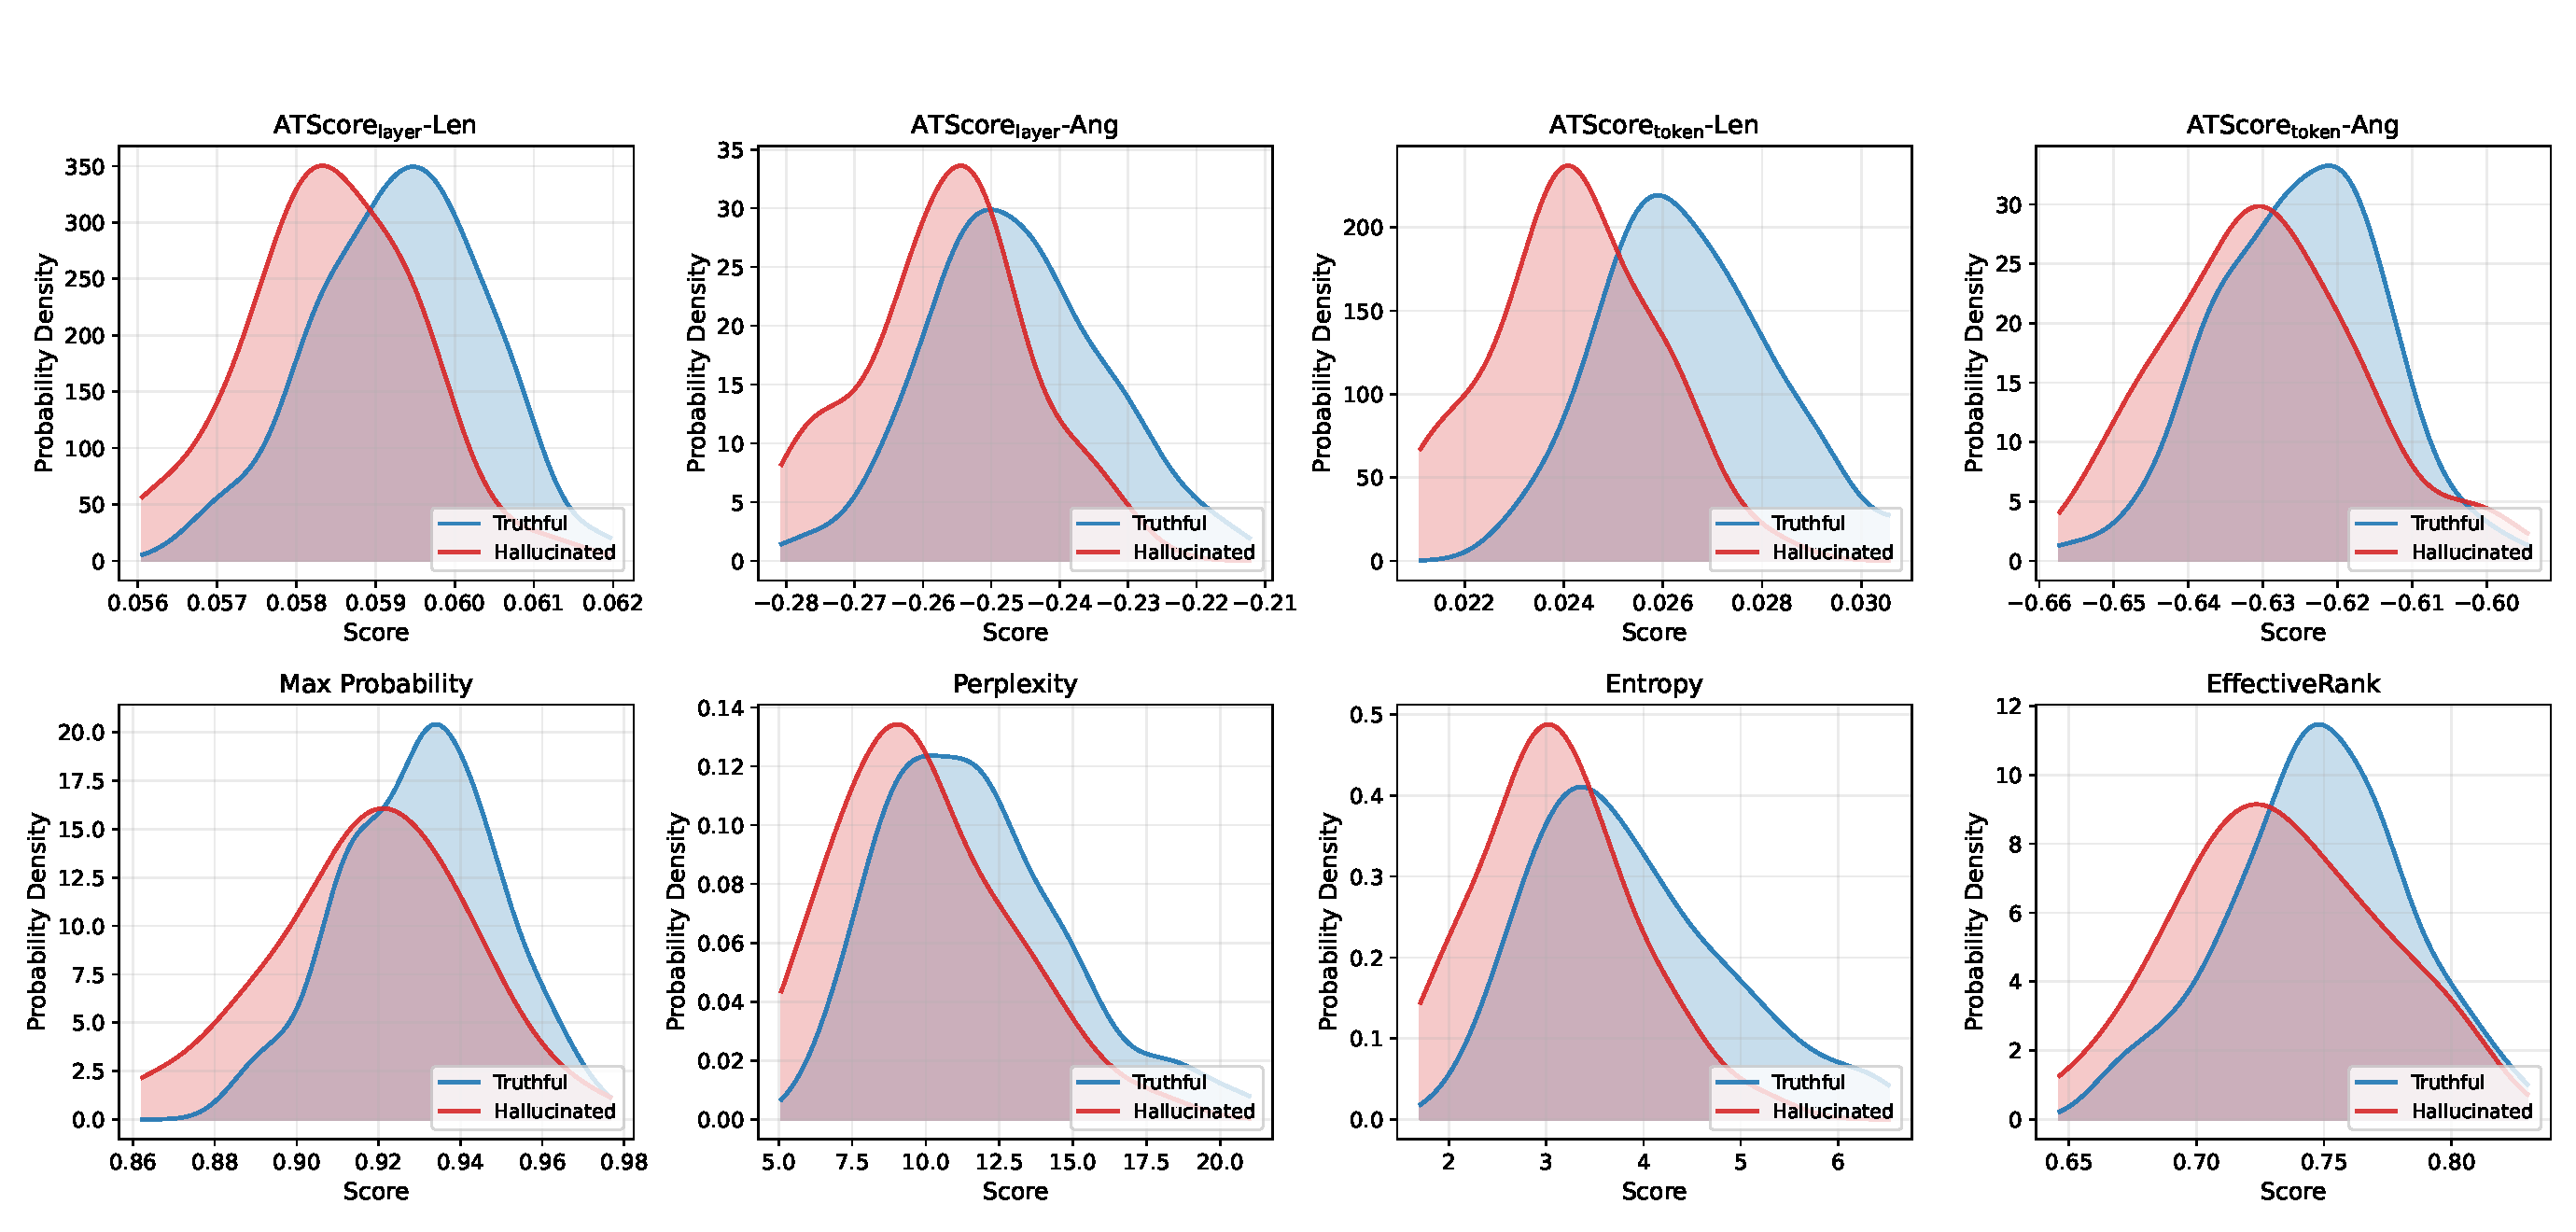
\includegraphics[width=\textwidth]{figures/content/coe_distribution_mgsm_Llama-3-8B-Instruct_en.pdf}
    \caption{ATScore和对比方法在GSM8K（MGSM）上的幻觉分数分布}\label{fig:distribution_mgsm}
\end{figure}

\begin{figure}[htb]
    \centering
    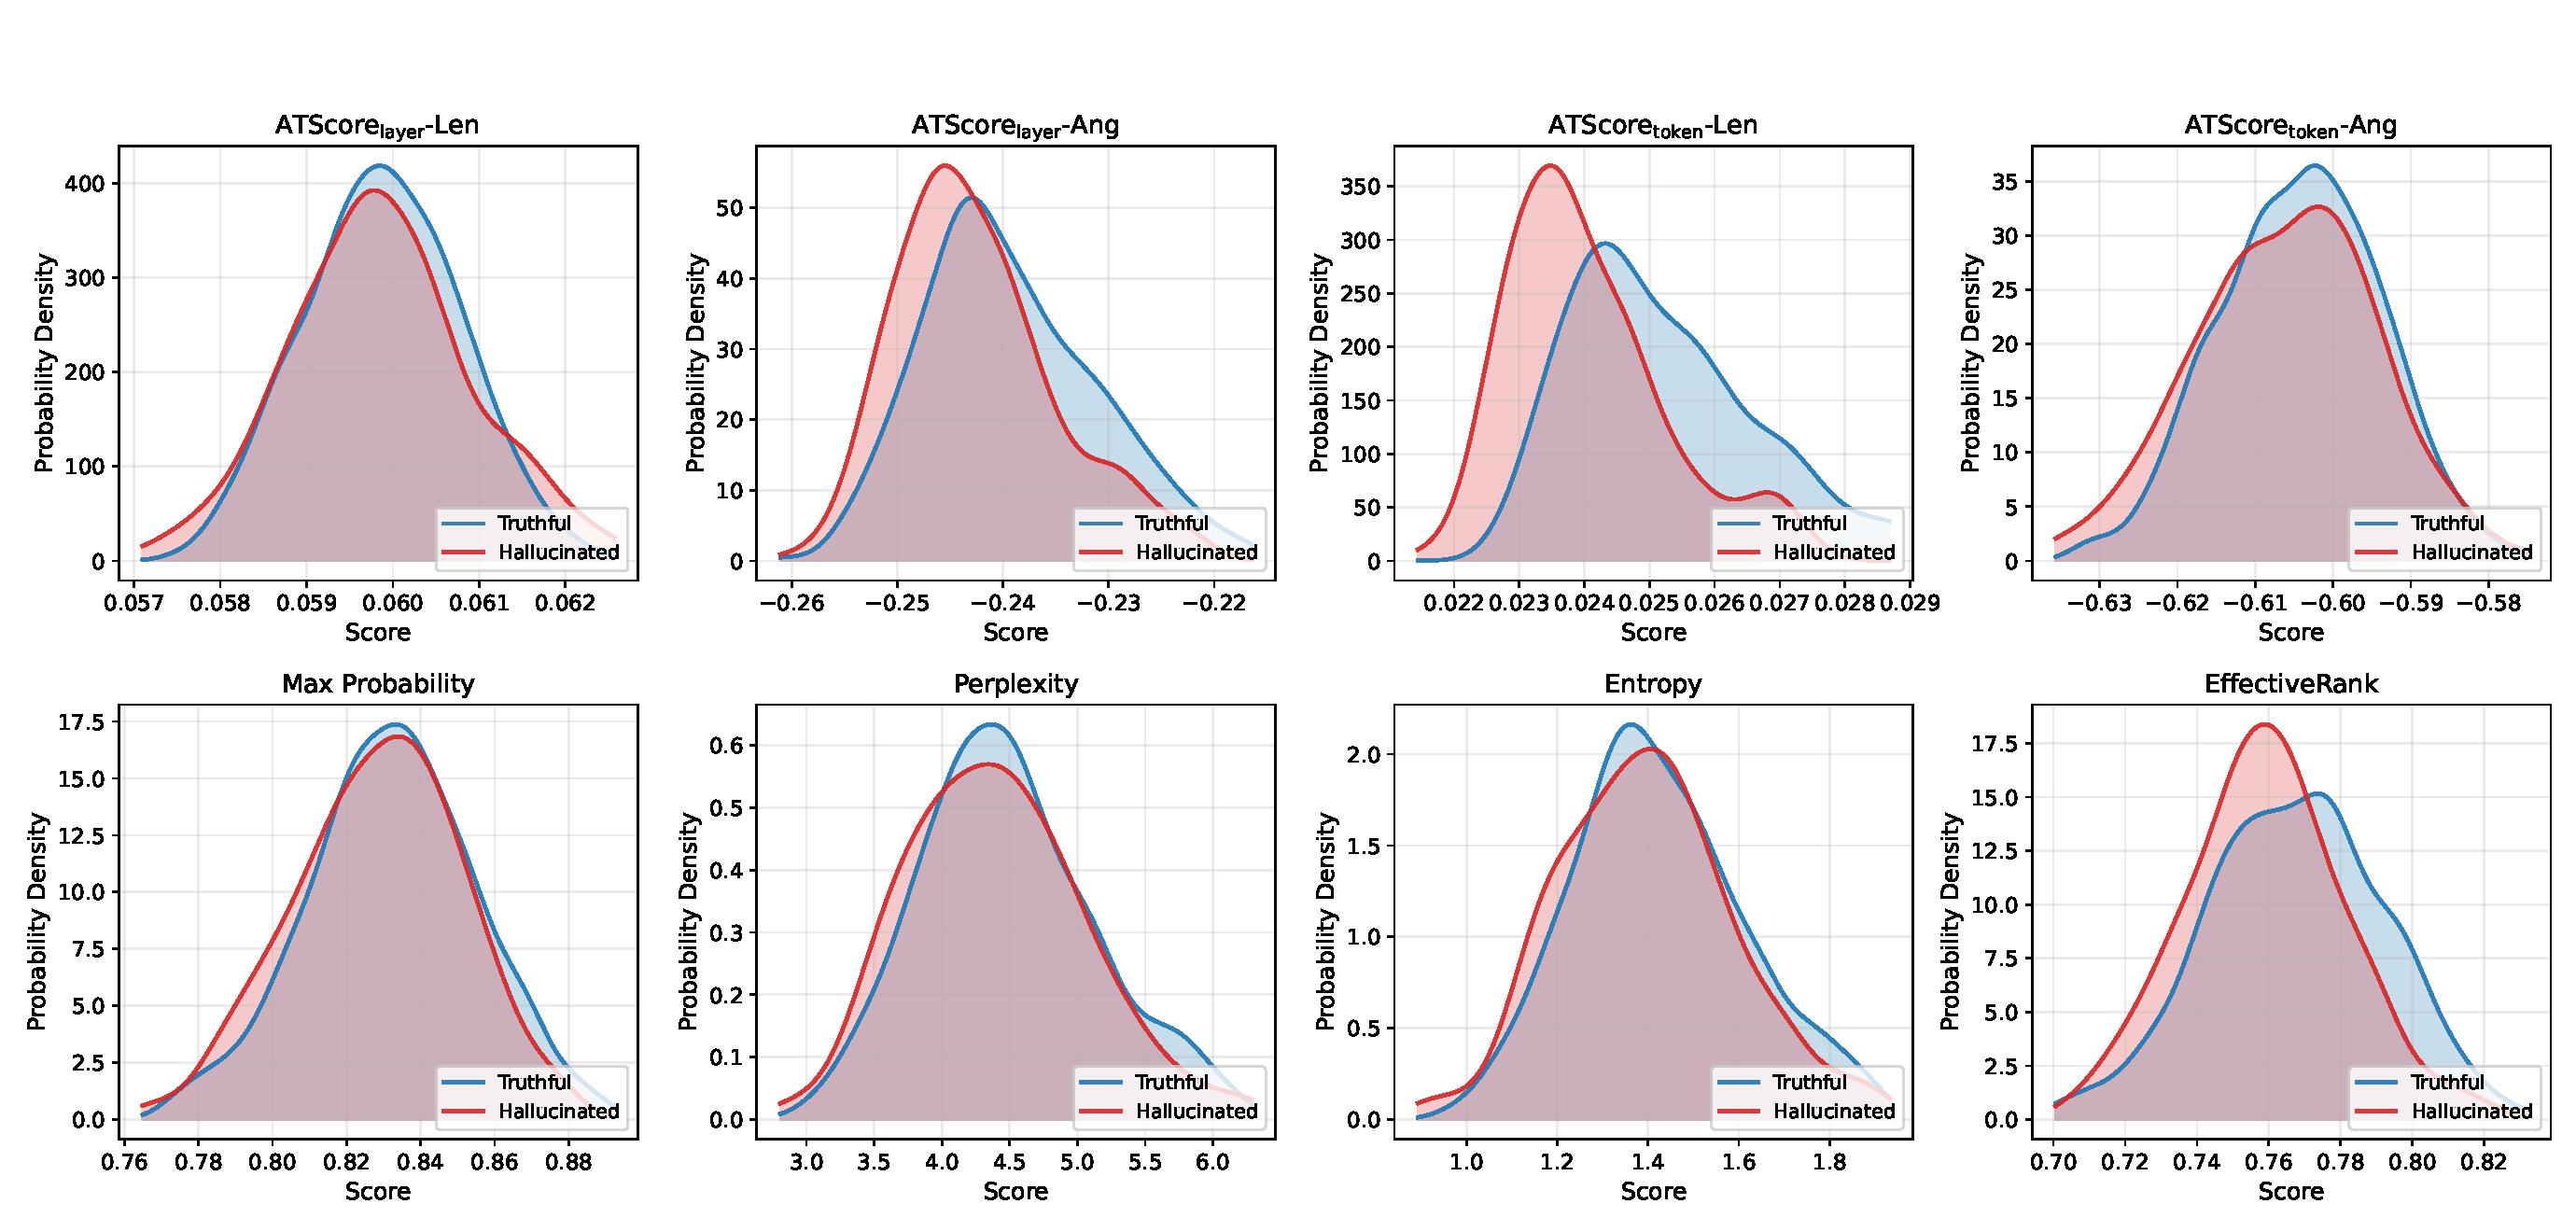
\includegraphics[width=\textwidth]{figures/content/coe_distribution_commonsenseqa_Llama-3-8B-Instruct_en.pdf}
    \caption{ATScore和对比方法在CommonsenseQA上的幻觉分数分布}\label{fig:distribution_csqa}
\end{figure}

从图中可以看出，ATScore系列方法整体上较黑盒统计量方法与传统白盒表征统计方法展现出更清晰的双峰分离趋势，其中ATScore$_{\mathrm{token}}$-Len在两个数据集上表现尤为突出：其真实回答与幻觉回答两组样本的密度峰位置偏移更明显，重叠区域相对更小，说明该方法能够更稳定地捕捉幻觉生成过程中内部表征轨迹的异常变化。这一现象与主实验结果是一致的，即ATScore系列在多数数据集及指标设定下取得最优，而ATScore$_{\mathrm{token}}$-Len则是整体表现最稳定、最优次数最多的变体。综合来看，这些分布图从可视化角度进一步验证了本文方法的有效性，也说明ATScore$_{\mathrm{token}}$-Len能够更充分地利用内部表征中的多方向结构信息，是本文最具代表性的主推方法。

从机制层面看，本文方法之所以能够取得较好的检测效果，主要源于其对大语言模型内部表征动态结构的更充分利用。传统黑盒方法主要依赖输出层概率或序列级似然信息，这类信号虽然计算简单，但往往只能反映最终输出的不确定性，难以深入揭示模型内部生成机制。幻觉的产生并不一定只在最终输出阶段才显现，其对应的异常模式往往会提前体现在隐藏状态的演化过程中。

本文方法通过构建链式表征，将原本分散在激活张量中的高维状态组织为具有顺序结构的表示轨迹，从而保留了内部状态随深度或随生成过程推进的动态变化信息。另一方面，链平均长度长、平均转折角度等几何指标具有较强的可解释性，能够分别从累计变化幅度、局部方向偏折和整体路径形态等角度刻画内部表征的异常程度。这种从“几何轨迹”视角出发的检测方式，不仅能够补充传统静态谱特征方法的信息不足，也使得所得到的幻觉分数具备更清晰的结构含义。综合来看，本文方法在无需额外训练或参数微调的前提下，仅通过对内部表征进行轻量级的方向聚合与几何统计即可实现有效检测，因而兼具较好的检测性能、可解释性与实际应用价值。

\subsection{消融实验}\label{subsec:ablation}

本小节将进一步对ATScore的各种变体，以及开放式问题的“真实/幻觉”标签判断方式进行详细的消融分析。

\subsubsection{辅助方向的聚合方式}

在~\ref{subsec:multi_direction_chain_representation}中，本文讨论了将激活张量分为两个正交的“主-次”方向：其中主方向保留链式顺序结构，另一辅助方向进行压缩聚合。对辅助方向的聚合方式有取辅助方向各元素之平均（avg，如$\phi_t^{\mathrm{avg}}=\frac{1}{T}\sum_{t=1}^{T}\mathbf{a}_{\ell,t}$与$\phi_{\ell}^{\mathrm{avg}}=\frac{1}{L}\sum_{\ell=1}^{L}\mathbf{a}_{\ell,t}$）与取末位置元素（last，如$\phi_t^{\mathrm{last}}=\mathbf{a}_{\ell,T}$与$\phi_{\ell}^{\mathrm{last}}=\mathbf{a}_{L,t}$）两种。表~\ref{tab:mgsm_avg_last}与表~\ref{tab:truthfulqa_avg_last}展示了在不同数据集上两种聚合方式的相对优劣。

\begin{table}[htbp]
  \centering
  \caption{ATScore在GSM8K（MGSM）数据集上不同辅助方向聚合方式的性能}
  \label{tab:mgsm_avg_last}
  \begin{autofittabular}{lccc}
  \toprule
  方法及辅助方向聚合方式 & AUROC~$\uparrow$（\%） & FPR95~$\downarrow$（\%） & AUPR~$\uparrow$（\%） \\
  \midrule
  ATScore$_{\mathrm{token}}$-Len（last）  & \textbf{69.22}	& \textbf{81.82}	& 90.27 \\
  ATScore$_{\mathrm{token}}$-Ang（last）  & 62.31	& 86.36	& 86.71 \\
  \midrule
  ATScore$_{\mathrm{token}}$-Len（avg）   & 69.00	& \textbf{81.82}	& \textbf{90.30} \\
  ATScore$_{\mathrm{token}}$-Ang（avg）   & 51.24	& 100.00 & 82.54 \\
  \bottomrule
  \end{autofittabular}
\end{table}

\begin{table}[htbp]
  \centering
  \caption{ATScore在TruthfulQA数据集上不同辅助方向聚合方式的性能}
  \label{tab:truthfulqa_avg_last}
  \begin{autofittabular}{lccc}
  \toprule
  方法及辅助方向聚合方式 & AUROC~$\uparrow$（\%） & FPR95~$\downarrow$（\%） & AUPR~$\uparrow$（\%） \\
  \midrule
  ATScore$_{\mathrm{token}}$-Len（last）  & \textbf{50.90}	& \textbf{91.18}	& \textbf{35.30} \\
  ATScore$_{\mathrm{token}}$-Ang（last）  & 49.33	& 93.43	& 33.36 \\
  \midrule
  ATScore$_{\mathrm{token}}$-Len（avg）   & 49.89	& 91.56	& 34.66 \\
  ATScore$_{\mathrm{token}}$-Ang（avg）   & 48.32	& 94.00	& 33.06 \\
  \bottomrule
  \end{autofittabular}
\end{table}

从表~\ref{tab:mgsm_avg_last}与表~\ref{tab:truthfulqa_avg_last}可以看出，在不同数据集上，采用末位置聚合（last）的整体性能通常优于平均聚合（avg），这一趋势在AUROC与FPR95等主要指标上表现得较为一致。特别是在链平均长度（Len）指标下，last与avg在部分情况下数值接近，但last往往仍能取得更优或更稳定的结果；而在链平均转折角度（Ang）指标下，last的优势更加明显，说明辅助方向聚合方式对链式表征的几何特性具有一定影响。

这一现象可以从内部表征的信息分布角度进行解释。在大语言模型的生成过程中，不同层或不同token位置的隐藏状态并非同等重要，末位置的表征通常更直接地参与当前token的生成决策，因而包含了更强的语义与置信信息。因大语言模型的自回归（auto-regressive）式生成本质，末位置的token理论上可与所有输入及已生成的token计算自注意力，因而更可能完整地包含句子级信息。相比之下，简单的平均聚合会在一定程度上引入无关或噪声信息，从而削弱链式表征中与幻觉相关的判别信号。

此外，链式建模依赖于相邻状态之间的变化来刻画表示轨迹的几何特性，而末位置聚合能够更突出该关键位置的状态差异，使得链长、角度等指标对异常变化更加敏感。因此，采用last作为辅助方向的聚合方式，能够在保留主要判别信息的同时减少信息稀释，从而在整体上取得更优的检测效果。

\subsubsection{开放式问题的“真实/幻觉”标签判定方式}

在~\ref{subsec:experiment_settings}中，本文讨论了对于模型输出的“真实/幻觉”标签的判定方式，此标签将被进一步应用于计算各幻觉检测算法的评价指标。由于自然语言的表达多样性，对于开放式问题，判定模型输出与参考答案是否相符（即是否幻觉），存在一定模糊空间。本文采取了基于字符级别匹配的ROUGE-L算法和基于大模型裁判（LLM judge）的两种判定方法，其中ROUGE-L相似度阈值取为$0.5$。在TruthfulQA这一开放式问答数据集上，本文所提出的方法的性能如表~\ref{tab:truthfulqa_rouge_llm_judge}所示。

\begin{table}[htbp]
  \centering
  \caption{ATScore在TruthfulQA数据集上基于不同判定幻觉标签方法的性能}
  \label{tab:truthfulqa_rouge_llm_judge}
  \begin{autofittabular}{clccc}
  \toprule
  判定标签方式 & 方法 & AUROC~$\uparrow$（\%） & FPR95~$\downarrow$（\%） & AUPR~$\uparrow$（\%） \\
  \midrule
  \multirow{6}{*}{\makecell{LLM Judge\\（幻觉率：65.2\%）}}  & R-MHP  & 47.84 & 94.93 & 32.96 \\
                              & EffectiveRank & 50.18	& 91.99	& \textbf{35.54} \\
                              \cmidrule{2-5}
                              & ATScore$_{\mathrm{layer}}$-Len  & 49.03	& 96.62	& 34.93 \\
                              & ATScore$_{\mathrm{layer}}$-Ang  & 48.88	& 95.12	& 34.39 \\
                              & ATScore$_{\mathrm{token}}$-Len  & \textbf{50.90}	& \textbf{91.18}	& 35.30 \\
                              & ATScore$_{\mathrm{token}}$-Ang  & 49.33	& 93.43	& 33.36 \\
  \midrule
  \multirow{6}{*}{\makecell{ROUGE-L\\（幻觉率：53.7\%）}}    & R-MHP  & 44.83 & 96.36	& 42.18 \\
                              & EffectiveRank & 49.22	& 95.22	& 46.59 \\
                              \cmidrule{2-5}
                              & ATScore$_{\mathrm{layer}}$-Len  & 49.69	& \textbf{92.71}	& 44.74 \\
                              & ATScore$_{\mathrm{layer}}$-Ang  & 46.34	& 99.09	& 44.65 \\
                              & ATScore$_{\mathrm{token}}$-Len  & 49.73	& 96.58	& 46.46 \\
                              & ATScore$_{\mathrm{token}}$-Ang  & \textbf{53.02} & 96.13	& \textbf{47.57} \\
  \bottomrule
  \end{autofittabular}
\end{table}

从表~\ref{tab:truthfulqa_rouge_llm_judge}中可以看出：不论采用何种方式构建用于计算评价指标的“真实/幻觉”标签，ATScore系列方法仍能在大多数情境下保持更高的性能。鉴于大模型更强的语义级别理解能力，基于大模型裁判判断的方法通常能够更准确地判断模型输出是否为幻觉，因此本文默认采用基于大模型裁判的判定方法。

\section{本章小结}

本章围绕大语言模型幻觉检测问题，在明确任务设定的基础上，提出了基于多方向表征建模的ATScore方法。该方法以大模型生成过程中的内部激活为切入点，构建三维激活张量，并分别从layer和token两个方向对其进行链式建模，再结合链长度、转折角度等几何指标实现对幻觉的有效检测。

实验结果表明，ATScore在多个数据集和多种评价指标上均具有良好的竞争力，整体优于多种黑盒与白盒基线方法，其中以token为主方向的变体表现更为突出。消融实验则进一步验证了辅助方向聚合方式以及标签判定策略对性能的影响。综合来看，本章方法在无需训练的条件下，充分利用了大模型内部表征中与幻觉相关的动态信号，展示了跨领域跨数据集的高泛化性能，为后续研究提供了方法基础。
